\documentclass{article}

\usepackage[utf8]{inputenc}  
\usepackage[T1]{fontenc}     
\usepackage{tikz}
\usetikzlibrary{shapes, positioning, arrows, calc}
\usetikzlibrary{decorations.pathreplacing}

\begin{document}

% Exemple tri

% état initial
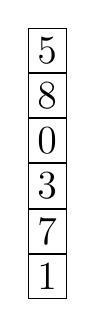
\begin{tikzpicture}
   \node [font=\sffamily\Large\bfseries, draw, anchor=center] (first) {$5$};
   \node [font=\sffamily\Large\bfseries, draw, anchor=center, below=0cm of first] (second) {$8$};
   \node [font=\sffamily\Large\bfseries, draw, anchor=center, below=0cm of second] (third) {$0$};
   \node [font=\sffamily\Large\bfseries, draw, anchor=center, below=0cm of third] (fourth) {$3$};
   \node [font=\sffamily\Large\bfseries, draw, anchor=center, below=0cm of fourth] (fifth) {$7$};
   \node [font=\sffamily\Large\bfseries, draw, anchor=center, below=0cm of fifth] (sixth) {$1$};
\end{tikzpicture}
\hspace{-0.25cm}
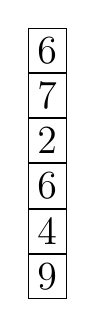
\begin{tikzpicture}
   \node [font=\sffamily\Large\bfseries, draw, anchor=center] (first) {$6$};
   \node [font=\sffamily\Large\bfseries, draw, anchor=center, below=0cm of first] (second) {$7$};
   \node [font=\sffamily\Large\bfseries, draw, anchor=center, below=0cm of second] (third) {$2$};
   \node [font=\sffamily\Large\bfseries, draw, anchor=center, below=0cm of third] (fourth) {$6$};
   \node [font=\sffamily\Large\bfseries, draw, anchor=center, below=0cm of fourth] (fifth) {$4$};
   \node [font=\sffamily\Large\bfseries, draw, anchor=center, below=0cm of fifth] (sixth) {$9$};
\end{tikzpicture}
% tour 1
\hspace{2cm}
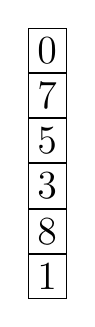
\begin{tikzpicture}
   \node [font=\sffamily\Large\bfseries, draw, anchor=center] (first) {$0$};
   \node [font=\sffamily\Large\bfseries, draw, anchor=center, below=0cm of first] (second) {$7$};
   \node [font=\sffamily\Large\bfseries, draw, anchor=center, below=0cm of second] (third) {$5$};
   \node [font=\sffamily\Large\bfseries, draw, anchor=center, below=0cm of third] (fourth) {$3$};
   \node [font=\sffamily\Large\bfseries, draw, anchor=center, below=0cm of fourth] (fifth) {$8$};
   \node [font=\sffamily\Large\bfseries, draw, anchor=center, below=0cm of fifth] (sixth) {$1$};
\end{tikzpicture}
\hspace{-0.25cm}
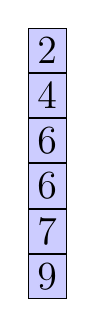
\begin{tikzpicture}
   \node [fill=blue!20, font=\sffamily\Large\bfseries, draw, anchor=center] (first) {$2$};
   \node [fill=blue!20, font=\sffamily\Large\bfseries, draw, anchor=center, below=0cm of first] (second) {$4$};
   \node [fill=blue!20, font=\sffamily\Large\bfseries, draw, anchor=center, below=0cm of second] (third) {$6$};
   \node [fill=blue!20, font=\sffamily\Large\bfseries, draw, anchor=center, below=0cm of third] (fourth) {$6$};
   \node [fill=blue!20, font=\sffamily\Large\bfseries, draw, anchor=center, below=0cm of fourth] (fifth) {$7$};
   \node [fill=blue!20, font=\sffamily\Large\bfseries, draw, anchor=center, below=0cm of fifth] (sixth) {$9$};
\end{tikzpicture}
% tour 2
\hspace{2cm}
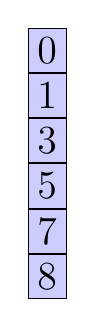
\begin{tikzpicture}
   \node [fill=blue!20, font=\sffamily\Large\bfseries, draw, anchor=center] (first) {$0$};
   \node [fill=blue!20, font=\sffamily\Large\bfseries, draw, anchor=center, below=0cm of first] (second) {$1$};
   \node [fill=blue!20, font=\sffamily\Large\bfseries, draw, anchor=center, below=0cm of second] (third) {$3$};
   \node [fill=blue!20, font=\sffamily\Large\bfseries, draw, anchor=center, below=0cm of third] (fourth) {$5$};
   \node [fill=blue!20, font=\sffamily\Large\bfseries, draw, anchor=center, below=0cm of fourth] (fifth) {$7$};
   \node [fill=blue!20, font=\sffamily\Large\bfseries, draw, anchor=center, below=0cm of fifth] (sixth) {$8$};
\end{tikzpicture}
\hspace{-0.25cm}
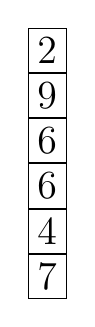
\begin{tikzpicture}
   \node [font=\sffamily\Large\bfseries, draw, anchor=center] (first) {$2$};
   \node [font=\sffamily\Large\bfseries, draw, anchor=center, below=0cm of first] (second) {$9$};
   \node [font=\sffamily\Large\bfseries, draw, anchor=center, below=0cm of second] (third) {$6$};
   \node [font=\sffamily\Large\bfseries, draw, anchor=center, below=0cm of third] (fourth) {$6$};
   \node [font=\sffamily\Large\bfseries, draw, anchor=center, below=0cm of fourth] (fifth) {$4$};
   \node [font=\sffamily\Large\bfseries, draw, anchor=center, below=0cm of fifth] (sixth) {$7$};
\end{tikzpicture}
% état final
\hspace{2cm}
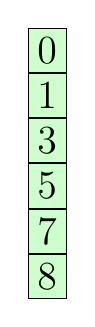
\begin{tikzpicture}
   \node [fill=green!20, font=\sffamily\Large\bfseries, draw, anchor=center] (first) {$0$};
   \node [fill=green!20, font=\sffamily\Large\bfseries, draw, anchor=center, below=0cm of first] (second) {$1$};
   \node [fill=green!20, font=\sffamily\Large\bfseries, draw, anchor=center, below=0cm of second] (third) {$3$};
   \node [fill=green!20, font=\sffamily\Large\bfseries, draw, anchor=center, below=0cm of third] (fourth) {$5$};
   \node [fill=green!20, font=\sffamily\Large\bfseries, draw, anchor=center, below=0cm of fourth] (fifth) {$7$};
   \node [fill=green!20, font=\sffamily\Large\bfseries, draw, anchor=center, below=0cm of fifth] (sixth) {$8$};
\end{tikzpicture}
\hspace{-0.25cm}
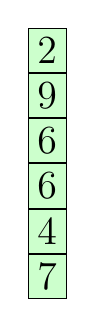
\begin{tikzpicture}
   \node [fill=green!20, font=\sffamily\Large\bfseries, draw, anchor=center] (first) {$2$};
   \node [fill=green!20, font=\sffamily\Large\bfseries, draw, anchor=center, below=0cm of first] (second) {$9$};
   \node [fill=green!20, font=\sffamily\Large\bfseries, draw, anchor=center, below=0cm of second] (third) {$6$};
   \node [fill=green!20, font=\sffamily\Large\bfseries, draw, anchor=center, below=0cm of third] (fourth) {$6$};
   \node [fill=green!20, font=\sffamily\Large\bfseries, draw, anchor=center, below=0cm of fourth] (fifth) {$4$};
   \node [fill=green!20, font=\sffamily\Large\bfseries, draw, anchor=center, below=0cm of fifth] (sixth) {$7$};
\end{tikzpicture}

% Explication tableau de files (implémentation)

\vspace{2cm}

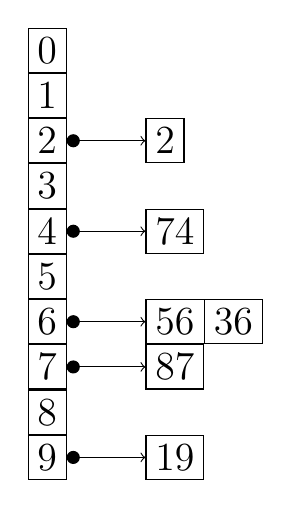
\begin{tikzpicture}
   \node [font=\sffamily\Large\bfseries, draw, anchor=center] (first) {$0$};
   \node [font=\sffamily\Large\bfseries, draw, anchor=center, below=0cm of first] (second) {$1$};
   \node [font=\sffamily\Large\bfseries, draw, anchor=center, below=0cm of second] (third) {$2$};
   \node [font=\sffamily\Large\bfseries, draw, anchor=center, below=0cm of third] (fourth) {$3$};
   \node [font=\sffamily\Large\bfseries, draw, anchor=center, below=0cm of fourth] (fifth) {$4$};
   \node [font=\sffamily\Large\bfseries, draw, anchor=center, below=0cm of fifth] (sixth) {$5$};
   \node [font=\sffamily\Large\bfseries, draw, anchor=center, below=0cm of sixth] (seventh) {$6$};
   \node [font=\sffamily\Large\bfseries, draw, anchor=center, below=0cm of seventh] (eighth) {$7$};
   \node [font=\sffamily\Large\bfseries, draw, anchor=center, below=0cm of eighth] (ninth) {$8$};
   \node [font=\sffamily\Large\bfseries, draw, anchor=center, below=0cm of ninth] (tenth) {$9$};

   \node [font=\sffamily\Large\bfseries, draw, anchor=center, right=1cm of third] (1) {$2$};
   \node [font=\sffamily\Large\bfseries, draw, anchor=center, right=1cm of fifth] (2) {$74$};
   \node [font=\sffamily\Large\bfseries, draw, anchor=center, right=1cm of seventh, rectangle split, rectangle split parts=2, rectangle split horizontal] (3)
         {$56$\nodepart{two}$36$};
   \node [font=\sffamily\Large\bfseries, draw, anchor=center, right=1cm of eighth] (4) {$87$};
   \node [font=\sffamily\Large\bfseries, draw, anchor=center, right=1cm of tenth] (5) {$19$};

   \draw[*->] (third) -- (1);
   \draw[*->] (fifth) -- (2);
   \draw[*->] (seventh) -- (3);
   \draw[*->] (eighth) -- (4);
   \draw[*->] (tenth) -- (5);
\end{tikzpicture}

\end{document}
